\chapter{Dark Matter candidate}
\label{chapter:candidate}

As discussed in \autoref{Chapter:introduction}, the key to find if a particle is a viable candidate for Dark Matter or not, is to check whether a particle is coupled or decoupled from the thermal bath, and calculate its abundance. 

In order to understand the thermal evolution of the universe, we need to compare the interaction rate, with the rate of expansion. 

The interactions of the particles occur within a homogeneous and isotropic gaseous equilibrium, we denominate this as the thermal bath. 
If the interactions are rapid enough to adjust to the changing of the temperature of the expanding universe, we can maintain our universe in a nearly thermal equilibrium.
The particles that remain in equilibrium with the thermal bath are denominated as being coupled with the thermal bath, and the ones that leave the equilibrium, are decoupled from the thermal bath.

We can say that a particle is either coupled or decoupled with the thermal bath, by the relation between the rate of interaction of said particle, $\Gamma$, and the rate of expansion of the universe, $H$
\begin{align}
	\label{eq}
	\begin{array}{ll}
		\Gamma > H \quad (coupled) \\
		\Gamma < H \quad (decoupled)
	\end{array}
\end{align}


\section{Interaction rate}

In this section, we are going to check if the pseudo-Goldstone boson studied in \autoref{chapter:Ultralight Bosons} is a viable candidate for DM.

The rate of interaction is given by
\begin{equation}
	\Gamma = n\langle \sigma v \rangle\,,
\end{equation}
where $n$ is the number density of our particle.

For the rate of interaction of pNGB we are only interested in the processes of annihilation $\theta+\theta \rightarrow SM + SM$, which were our main focus in Section \autoref{chapter:thermodynamicsofearlyuniverse}.
And so the rate of interaction is 
\begin{equation}
	\Gamma=\frac{g}{16m^2\pi^2K_2(m/T)}\int_{4m^2}^\infty\sigma(s-4m^2)\sqrt{s}K_1\left(\frac{\sqrt{s}}{T}\right)ds\,.
\end{equation}

To calculate the rate of interaction, we need to determine the cross-section of the reaction, $\sigma$ in \autoref{sigmav}, where the squared amplitude of the process, $|\mathcal{M}|^2$ in \autoref{crosssection}, was calculated using CalcHEP.

CalcHEP is a package for the calculation of Feynman diagrams \cite{Belyaev_2013}, implementing the model studied in the Section \autoref{chapter:Ultralight Bosons}, considering only the $s$-channels with mediators like the Higgs and $h_2$, where the $t$ and $u$ channels were not considered as they would have near to no impact on the amplitude of the process of annihilation of pGB.
And then for the calculation of the integrals, we used Cuba, a library for multidimensional numerical integration \cite{HAHN200578}, in C++ language.



For simplification reasons, we are going to make all the coupling terms, $\lambda_{H}$, $\lambda_{H\phi}$ and $\lambda_{\phi}$ constant which are bounded by the conditions in Eq.(\ref{couplingtermconditions}) and vary the VEV, $v_\sigma$, which is directly related to the mass of the Higgs.
If we recall the \autoref{masses}, we can manipulate both $h_1$ and $h_2$ masses, in order for one of them to equal the mass of the SM-Higgs and the other to have any values depending on $v_\sigma$.
And so we obtain the following rates of interaction 


\begin{figure}[H]
	\centering
	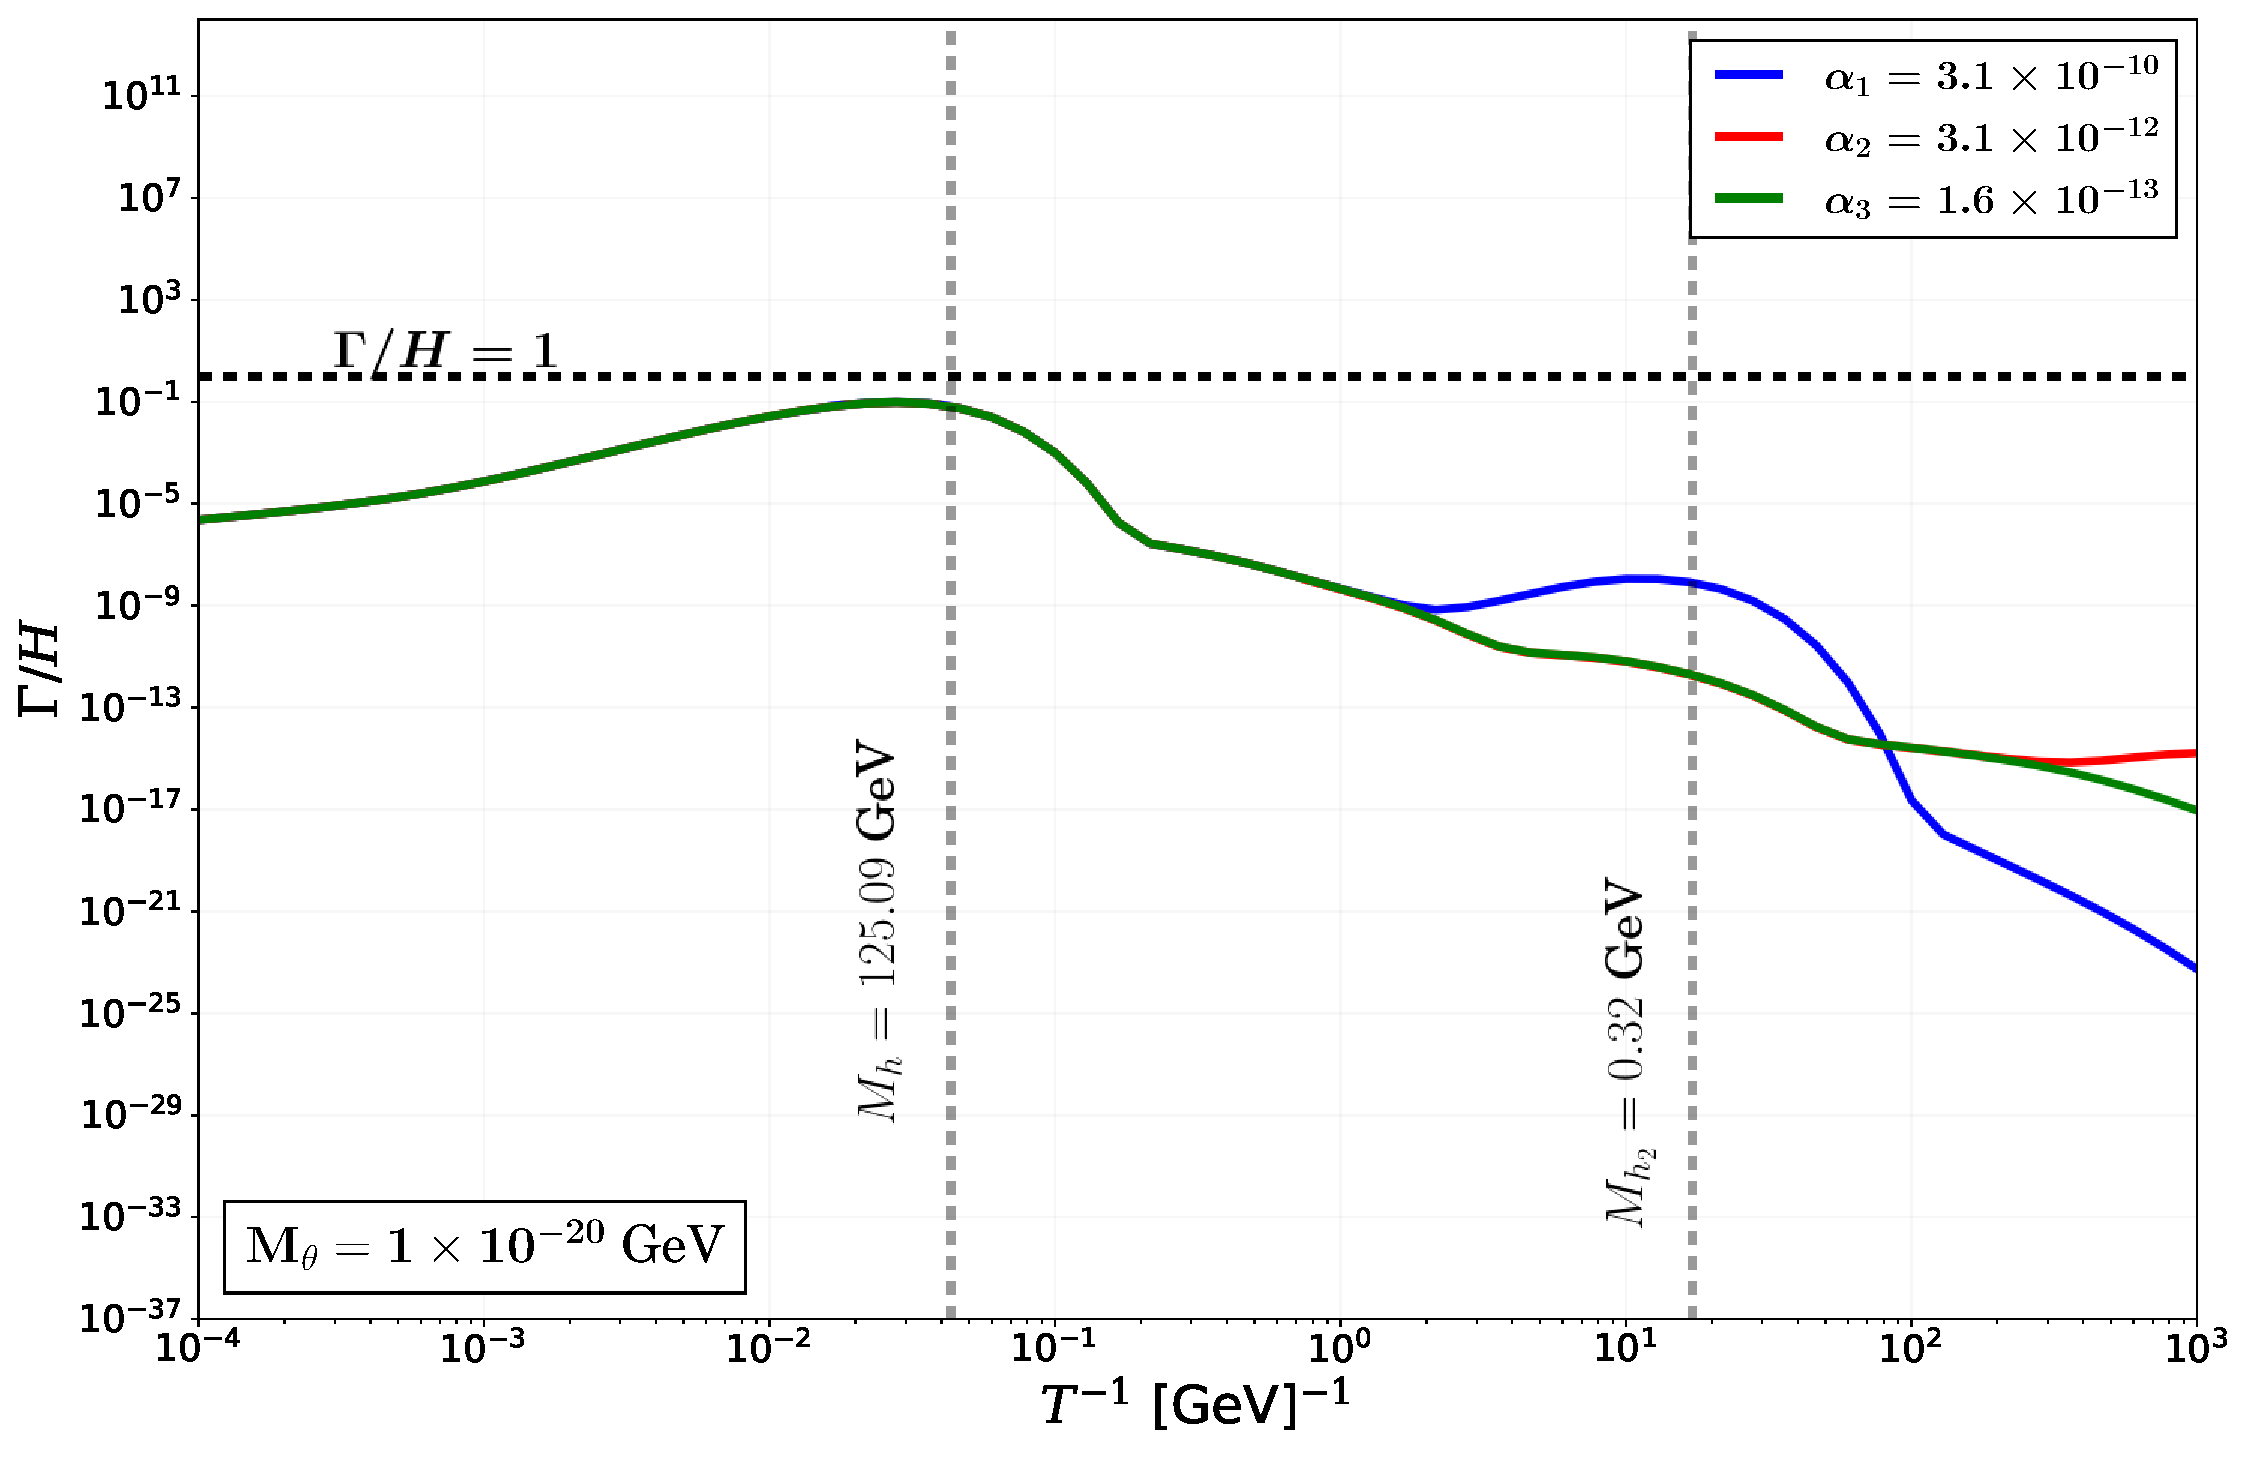
\includegraphics[width=0.7\linewidth]{graphs/ratedm_lesser}
	\caption{Rate of interaction divided by Hubble assuming $m_h \gg m_{h_2}$, for $\nu_\sigma=1$ \si{G\eV} ($M_{h_2} = 3.2\times10^{-1}$ \si{G\eV}),  $\nu_\sigma=0.01$ \si{G\eV} ($M_{h_2} = 3.2\times10^{-3}$ \si{G\eV}) and  $\nu_\sigma= 5\times10^{-4}$ \si{G\eV} ($M_{h_2} = 1.6\times10^{-4}$ \si{G\eV}), for blue, green and red curves, respectively.  Additionally, we have used $\lambda_H\sim0.26$, $\lambda_{H\phi}=2\times10^{-8}$ and $\lambda_\phi=0.1$\,.}
	\label{fig:ratelesser}
\end{figure}

\begin{figure}[H]
	\centering
	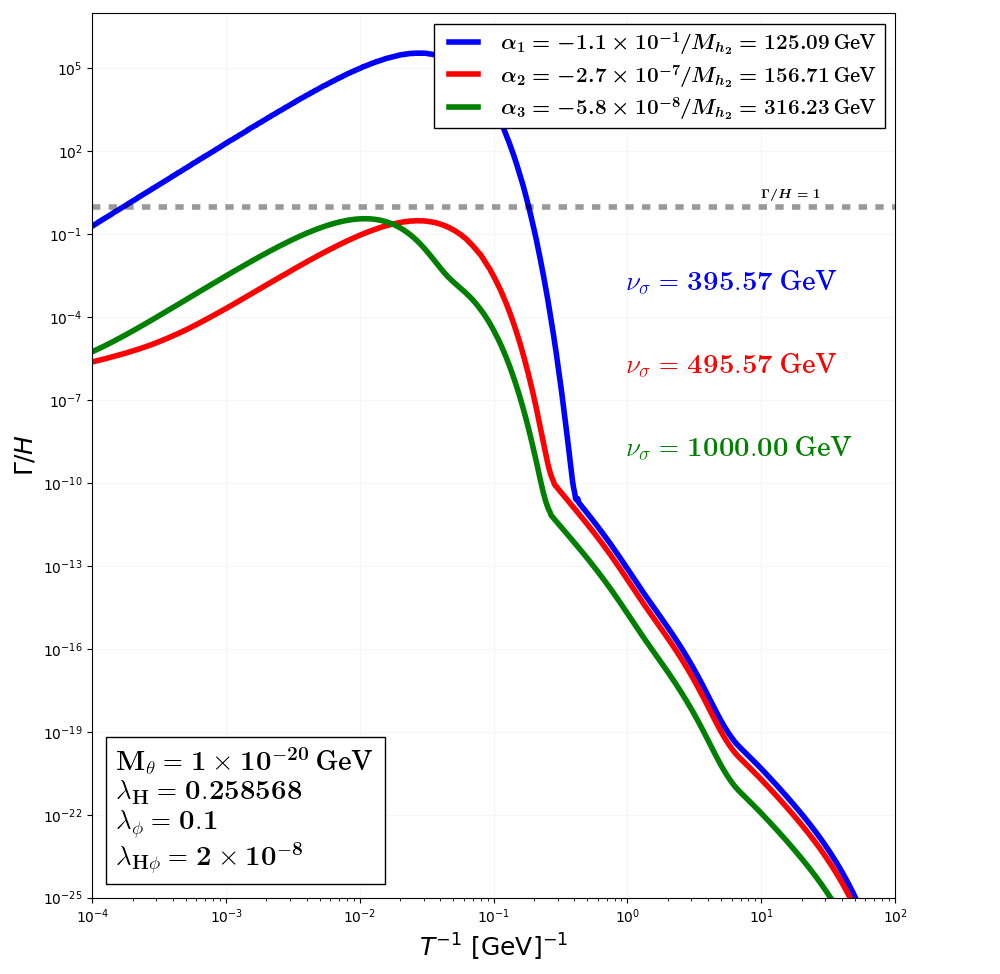
\includegraphics[width=0.75\linewidth]{graphs/ratedm_equal}
	\caption{Rate of interaction divided by Hubble assuming $m_h = m_{h_2}$, for $\nu_\sigma=395.57$ \si{G\eV} ($M_{h_2}=125.09$ \si{G\eV}),  $\nu_\sigma=495.57$ \si{G\eV} ($M_{h_2}=156.71$ \si{G\eV}) and  $\nu_\sigma=10^3$ \si{G\eV}  ($M_{h_2}=316.23$ \si{G\eV}), for blue, green and red curves, respectively.  Additionally, we have used $\lambda_H\sim0.26$, $\lambda_{H\phi}=2\times10^{-8}$ and $\lambda_\phi=0.1$\,.}
	\label{fig:rateequal}
\end{figure}

\begin{figure}[H]
	\centering
	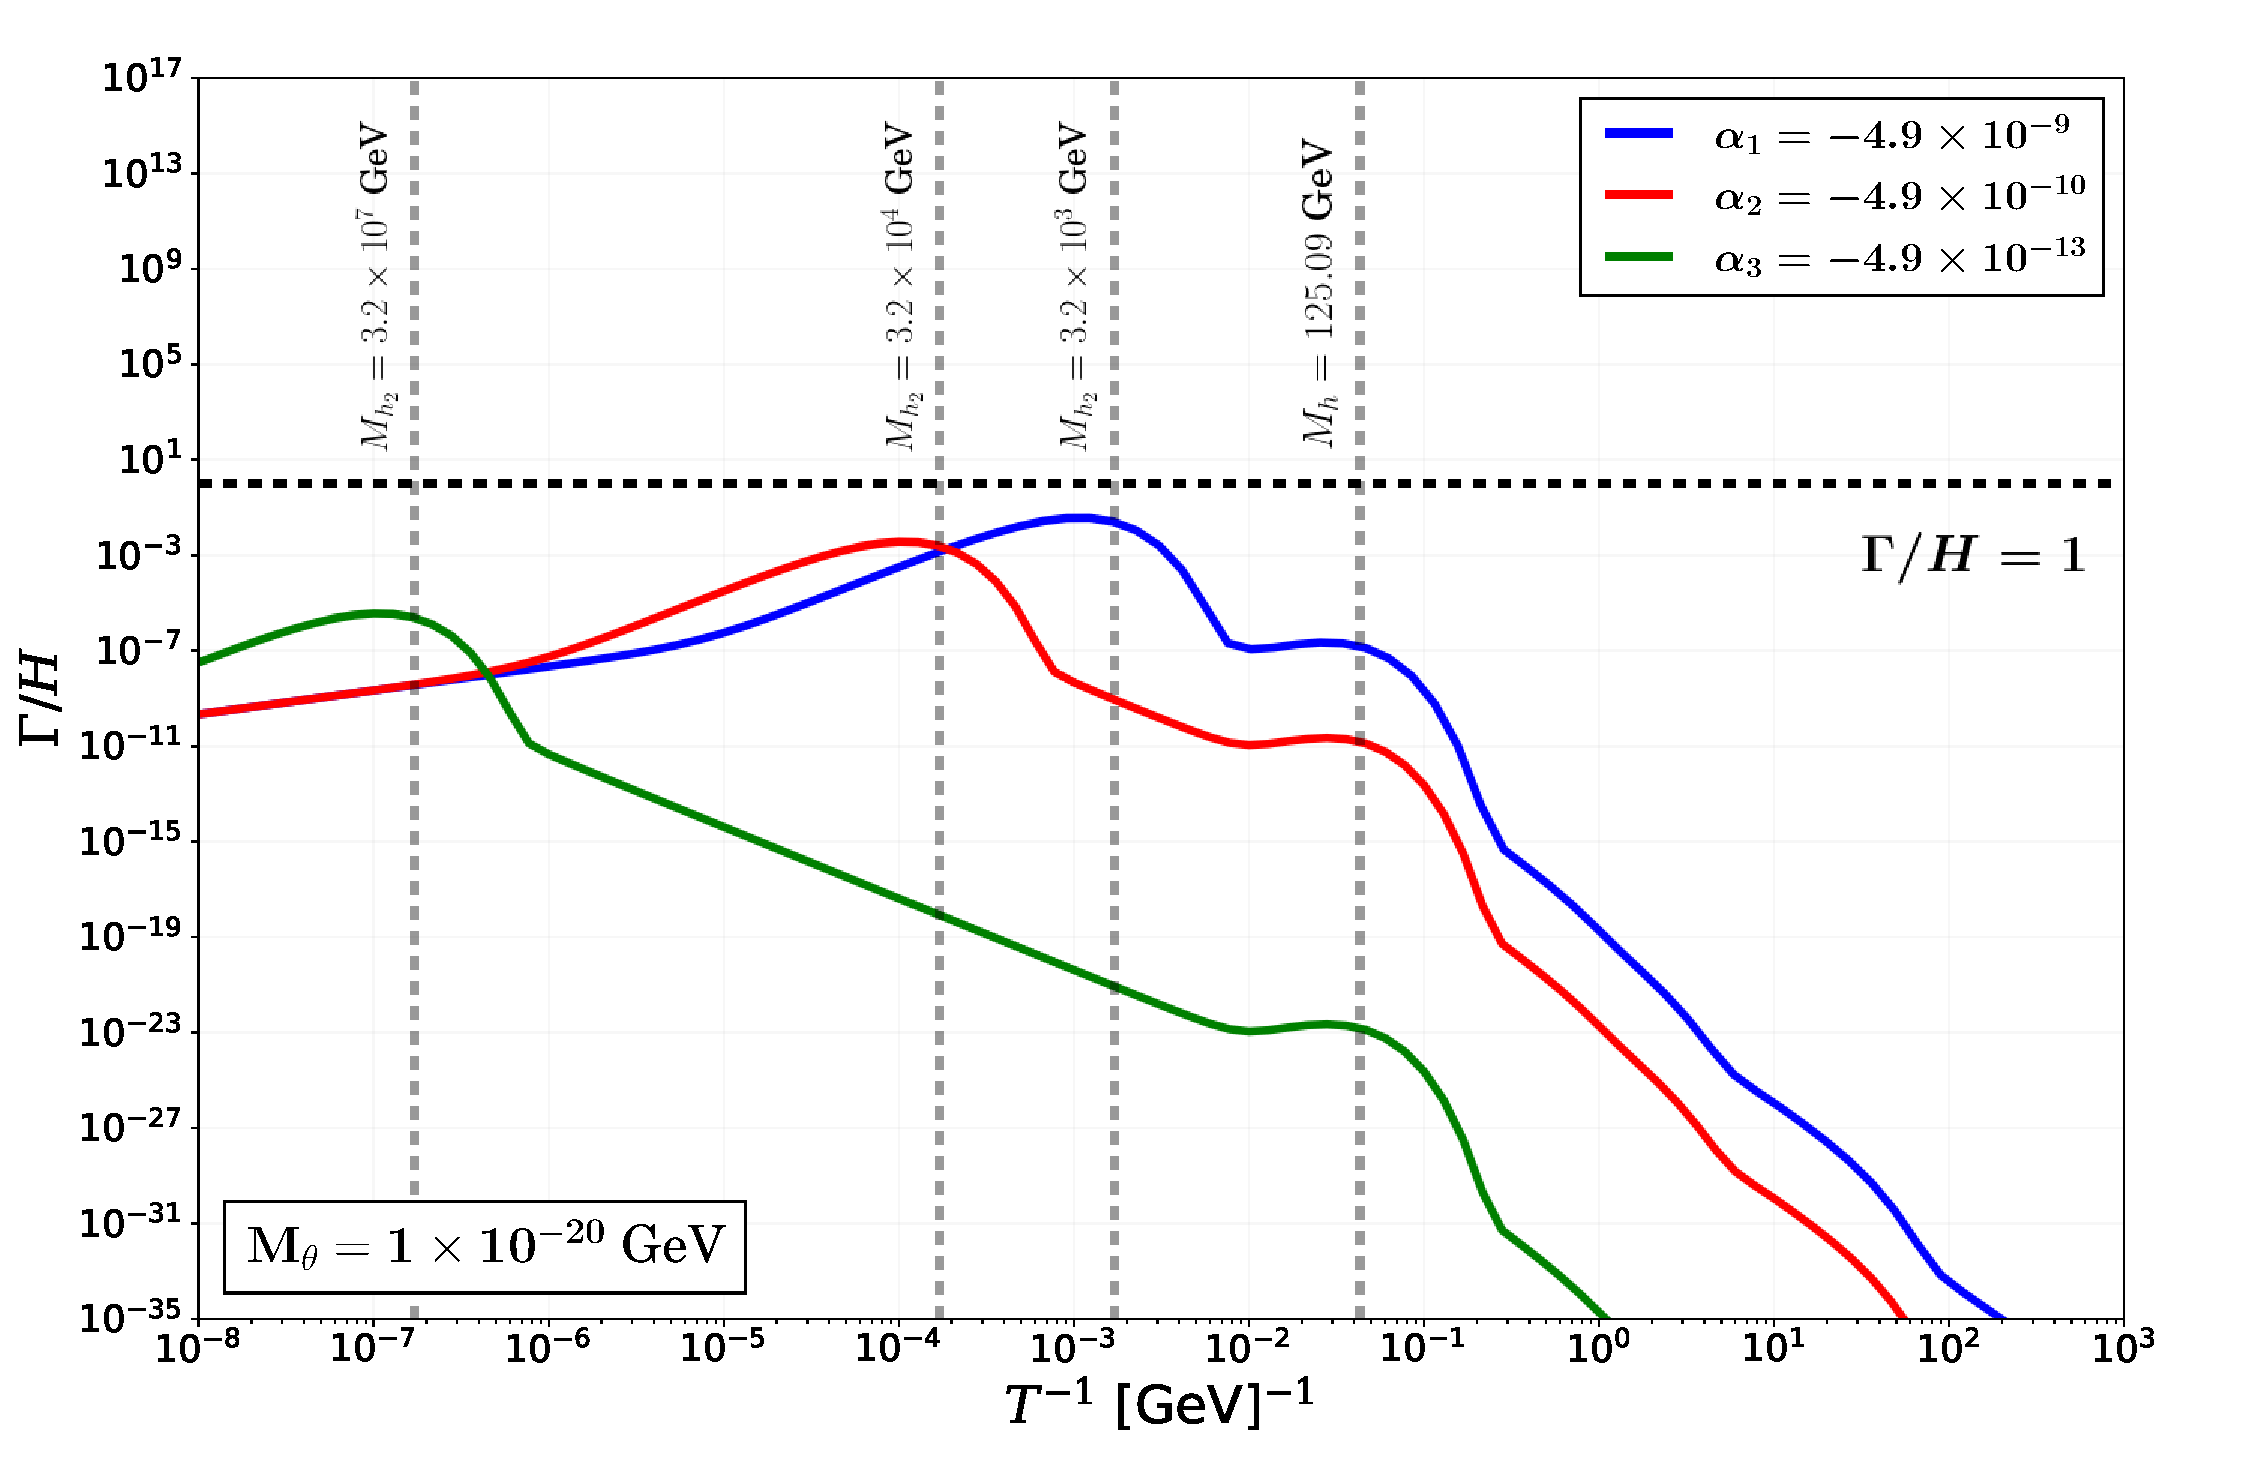
\includegraphics[width=0.8\linewidth]{graphs/ratedm_greater}
	\caption{Rate of interaction divided by Hubble assuming $m_h \ll m_{h_2}$, for $\nu_\sigma=10^4$ \si{G\eV} ($M_{h_2} = 3.2\times10^{3}$ \si{G\eV}),  $\nu_\sigma=10^5$ \si{G\eV} ($M_{h_2} = 3.2\times10^{4}$ \si{G\eV}) and  $\nu_\sigma= 10^8$ \si{G\eV} ($M_{h_2} = 3.2\times10^{7}$ \si{G\eV}), for blue, green and red curves, respectively.  Additionally, we have used $\lambda_H\sim0.26$, $\lambda_{H\phi}=2\times10^{-8}$ and $\lambda_\phi=0.1$\,.}
	\label{fig:rategreater}
\end{figure}

We can prove that as long as, the mixing angle, $\alpha\lesssim10^{-7}$, our pNGB doesn't couple with the thermal bath, and so doesn't become relativistic (cold). Notice that this constraint in the mixing angle, allows our VEV $v_\sigma$ to become a free parameter, as long as the quartic coupling terms remain the same. As mentioned in \autoref{chapter:Ultralight Bosons}, the mixing angle being small only allows decays of the $h_2$ into $\theta\theta$, and seeing as $v_\sigma$ becomes a free parameter, for large values of $v_\sigma$, this decay also disappears.

Note that there is a resonance whenever the temperature is approximately equal to the mass of the mediator, SM-Higgs or $h_2$, for $T\thicksim m_{h_{1,2}}/5.4$\cite{kolb}.

\section{Misalignment}
 
In this section, we are going to consider that the soft-symmetry breaking of the U$(1)_G$ symmetry, which produced the pNGB, occurred before the end of inflation. Inflation is a theory that explains the exponential rate of expansion of the early universe.

The temperature at which inflation occurred is bounded by the 

Using the \autoref{newvsoft}, and introducing the misalignment angle as $\Theta = \dfrac{2\theta}{v_\sigma}$
\begin{equation}
    V_{\textrm{soft}}(\Theta)\simeq \frac{m_\theta^2}{2}\left(\frac{v_\sigma}{2}\right)^2\Theta^2\,.
\end{equation}

Using the energy-momentum tensor, $T^{\mu}_\nu$, of $\theta$ 
\begin{equation}
    T^\mu_\nu=g^{\mu\alpha}(\partial_\alpha\theta)(\partial_\nu\theta)-\frac{\delta^\mu_\nu}{2}[g^{\alpha\beta}(\partial_\alpha\theta)(\partial_\beta\theta)+2V(\theta)]\,,
\end{equation}
where $g^{\mu\nu}=diag(-1,1,1,1)$ and the energy density reads as \cite{Marsh_2016}\cite{kolb}
\begin{align}
\label{densityenergy}
\begin{array}{ccc}
    &\rho_\theta=-T^0_0=-g^{0\alpha}(\partial_\alpha\theta)(\partial_0\theta)+\dfrac{1}{2}[g^{\alpha\beta}(\partial_\alpha\theta)(\partial_\beta\theta)+2V(\theta)]=\dfrac{1}{2}\left(\dfrac{\partial\theta}{\partial t}\right)^2-\dfrac{1}{2}\dfrac{\vec{\nabla}^2\theta}{a^2}+V(\theta)=\\ [5pt]
    &=\dfrac{1}{2}\left(\dfrac{\partial\theta}{\partial t}\right)^2+V(\theta)=\left(\dfrac{v_\sigma}{2}\right)^2\left[\dfrac{\dot{\Theta}^2}{2}+\dfrac{m_\theta^2}{2}\Theta^2\right]\,,
\end{array}
\end{align}
where $\theta$ only varies with time and is the same in the universe.

Knowing that the energy density of $\theta$ can be given by
\begin{equation}
\label{rhoa}
    \rho_\theta(a)=\rho_\theta(a_i)\left(\dfrac{a_i}{a}\right)^3\,,
\end{equation}
where $a$ is the scale factor, and the $a_i$ relates do any value of the scale factor.

In the radiation era of the universe, we have that, $a\propto \sqrt{t}$, where $t$ is the age of the universe.

The equation of motion for $\theta$ can be obtained varying the action, $S=\int \mathcal{L} a^3 d^4x$ , where $a$
is the scale factor, and computing the D’Alembertian for the Friedmann–Robertson–Walker (FRW) metric we obtain\cite{Marsh_2016}
\begin{equation}
\label{motion}
    \ddot{\Theta}^2+3H\dot{\Theta}+m_\theta^2\Theta=0\,.
\end{equation}

\begin{figure}[H]
	\centering
	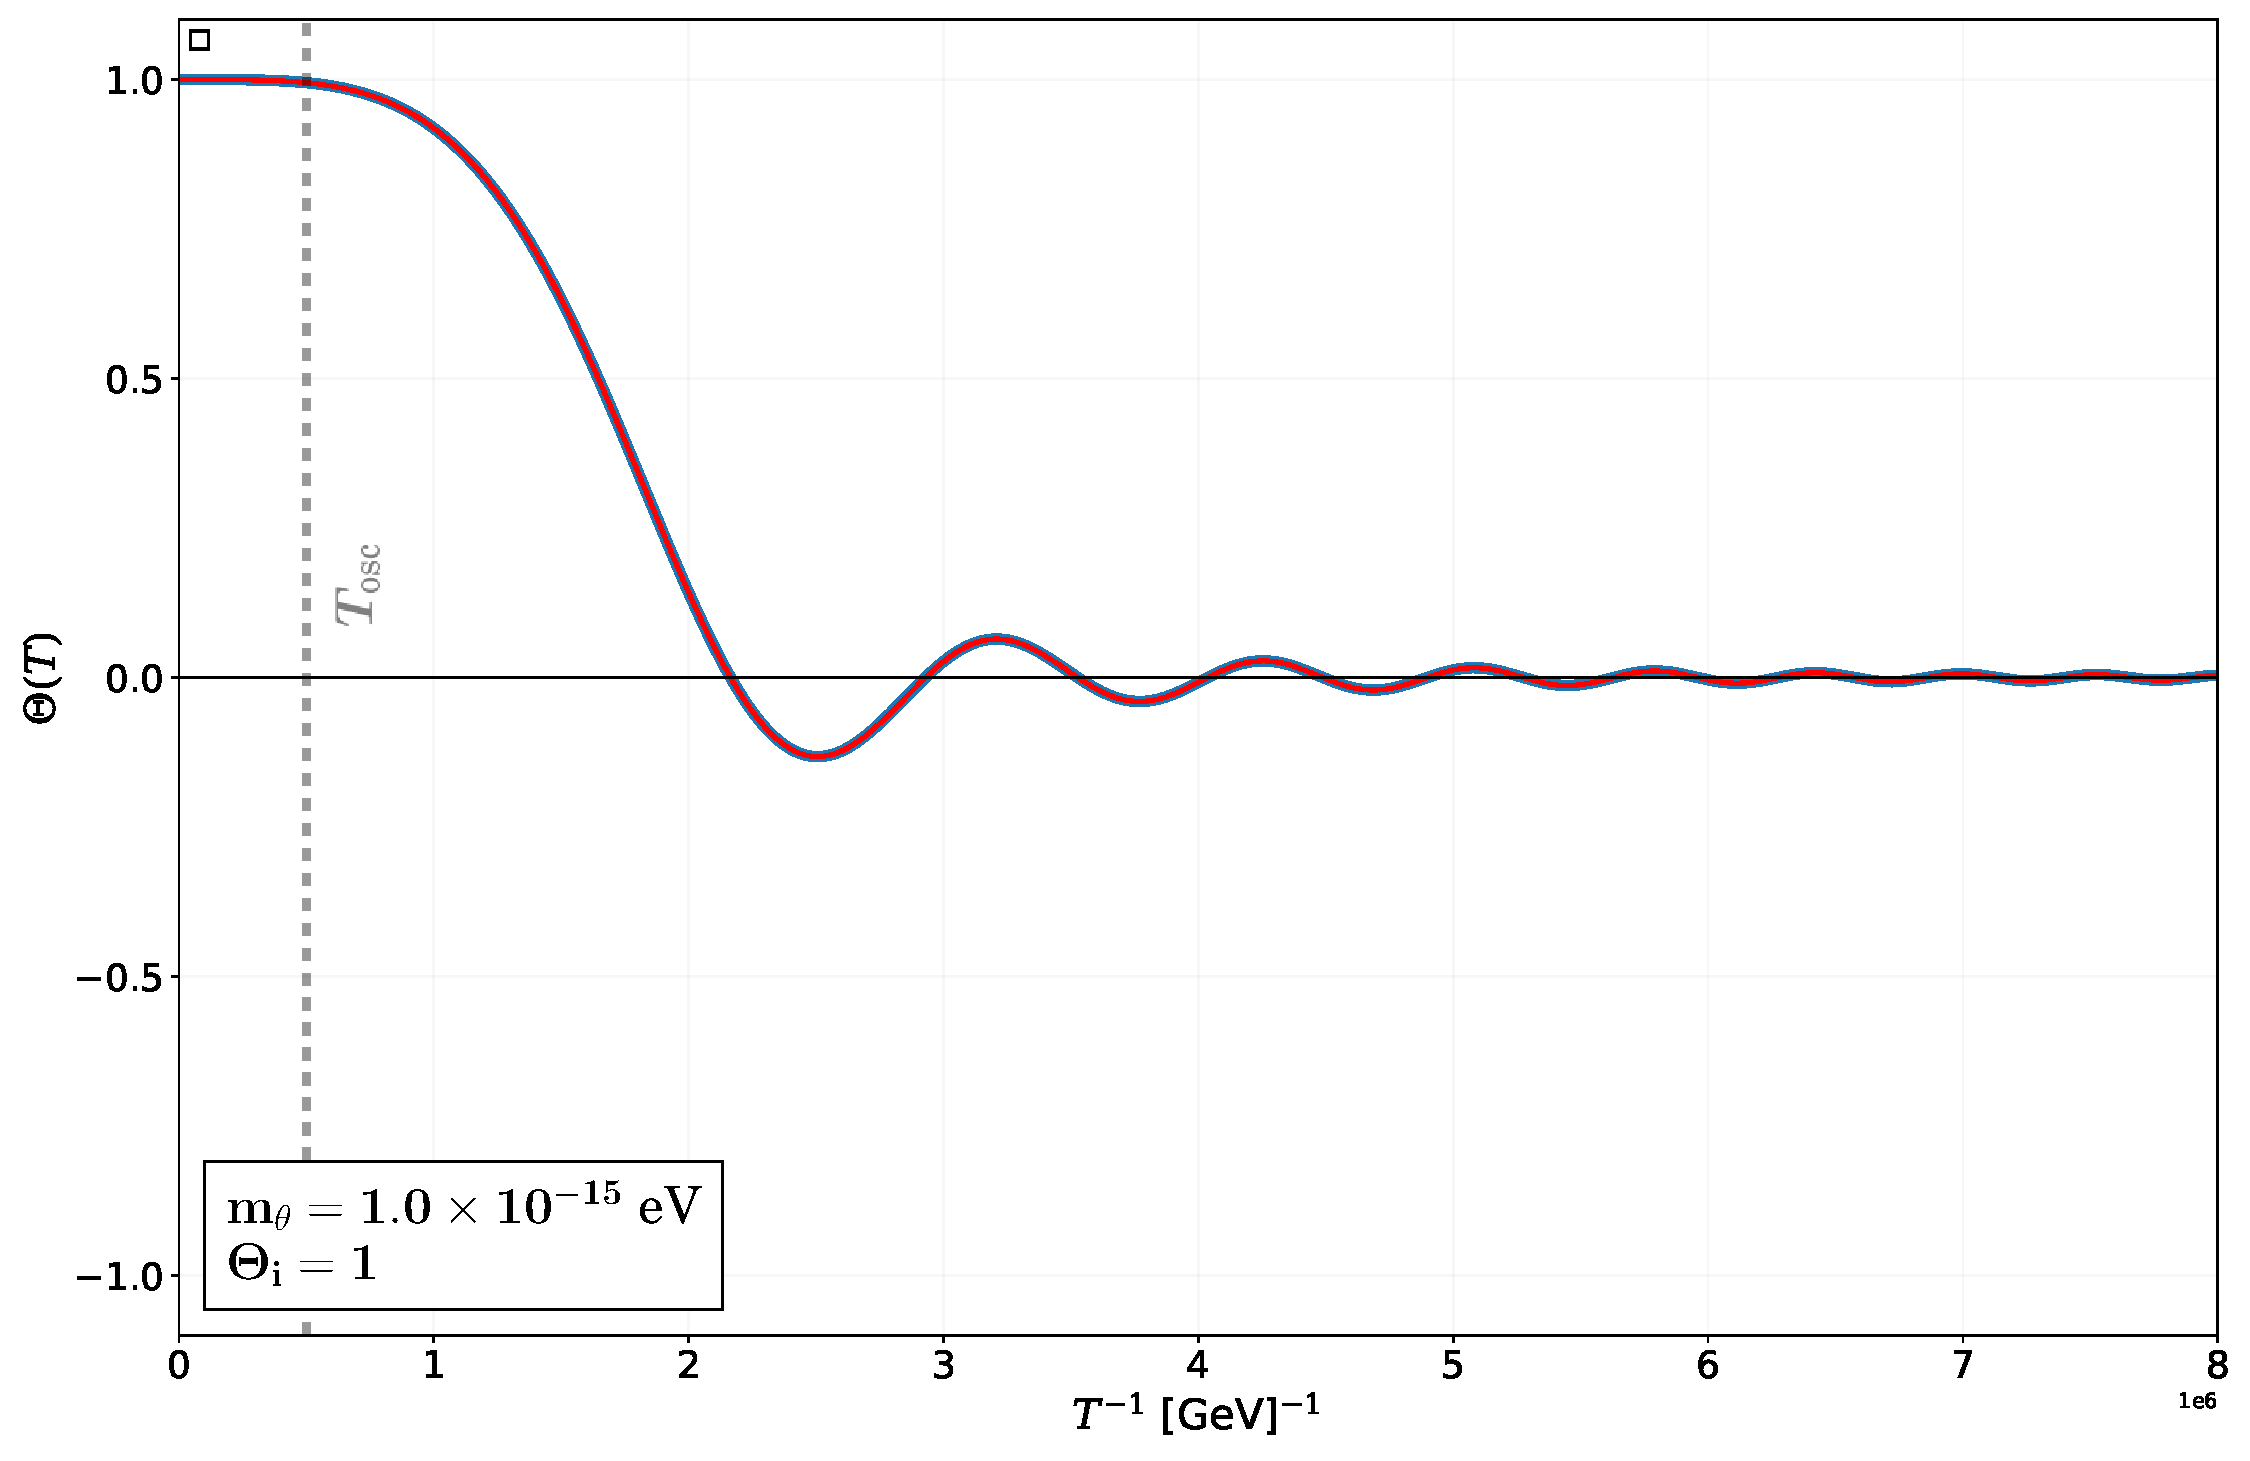
\includegraphics[width=0.9\linewidth]{graphs/motion.pdf}
	\caption{Solution of the equation of motion in \autoref{motion}\,.}
	\label{fig:motion}
\end{figure}

The \autoref{fig:motion}, allows us to see that the misalignment angle, $\Theta$, is constant for $T^{-1}\in[0,T^{-1}_{\textrm{osc}}]$, and so we can say from \autoref{densityenergy} that
\begin{equation}
    \rho_\theta(a_\textrm{osc})=\left(\dfrac{v_\sigma}{2}\right)^2\dfrac{m_\theta^2}{2}\Theta_\textrm{osc}^2\,.
\end{equation}

Using the \autoref{rhoa}, for an $a_i=a_\textrm{osc}$, we have
\begin{equation}
\label{rhoaa}
    \rho_\theta(a)=\left(\dfrac{v_\sigma}{2}\right)^2\dfrac{m_\theta^2}{2}\Theta_\textrm{osc}^2\left(\dfrac{a_\textrm{osc}}{a}\right)^3\,.
\end{equation}

Let us take a look at the entropy in the primordial universe, it can be written in terms of the pressure, $P$, and density of energy, $\rho$, as
\begin{equation}
    S=sa^3=\dfrac{\rho+P}{T}a^3\,,
\end{equation}
where $s$ is entropy density, recalling Equations (\ref{3.32}) and (\ref{eqn:3.16}) we have that the entropy can be written as
\begin{equation}
    S=\dfrac{2\pi^2}{45}g_{*s}(T)T^3a^3\,,
\end{equation}
where, $g_{*s}(T)$ is
\begin{equation}
	g_{*s}(T)=\sum\limits_{b}g_b\left(\frac{T_b}{T}\right)^3+\dfrac{7}{8}\sum\limits_{f}g_f\left(\frac{T_f}{T}\right)^3\,.
\end{equation}

Taking the following ratio,
\begin{equation}
\label{ratioS}
    \dfrac{S_\textrm{osc}}{S}=\dfrac{g_{*s}(T_\textrm{osc})}{g_{*s}(T)}\left(\dfrac{T_\textrm{osc}a_\textrm{osc}}{Ta}\right)^3\,,
\end{equation}
knowing that in the primordial universe the entropy is constant, so $S_\textrm{osc}=S$, the \autoref{ratioS} gets turned into
\begin{equation}
\label{aosc/a}
       \left(\dfrac{a_\textrm{osc}}{a}\right)^3=\dfrac{g_{*s}(T)}{g_{*s}(T_\textrm{osc})}\left(\dfrac{T}{T_\textrm{osc}}\right)^3\,.
\end{equation}

Using the \autoref{aosc/a}, the current energy density of $\theta$, in \autoref{rhoaa}, becomes
\begin{equation}
    \label{rhoaaa}
    \rho_\theta(a_0)=\left(\dfrac{v_\sigma}{2}\right)^2\dfrac{m_\theta^2}{2}\Theta_\textrm{osc}^2\dfrac{g_{*s}(T_0)}{g_{*s}(T_\textrm{osc})}\left(\dfrac{T_0}{T_\textrm{osc}}\right)^3\,.
\end{equation}
 
The current relic density of any matter is given by
\begin{equation}
    \Omega^0=\dfrac{\rho(a_0)}{\rho_\textrm{crit}}\,,
\end{equation}
and so using \autoref{rhoaaa}, the current relic density of $\theta$ reads as
\begin{equation}
    \Omega^0_\theta=\dfrac{\rho_\theta(a_0)}{\rho_\textrm{crit}}=\frac{1}{\rho_\textrm{crit}}\left(\dfrac{v_\sigma}{2}\right)^2\dfrac{m_\theta^2}{2}\Theta_\textrm{osc}^2\dfrac{g_{*s}(T_0)}{g_{*s}(T_\textrm{osc})}\left(\dfrac{T_0}{T_\textrm{osc}}\right)^3\,.
\end{equation}

This can be further simplified as we know most of this terms,  $\rho_\textrm{crit}=1.88\times 10^{-29}h^2 \si{\g\cm^{-3}}=8.1\times10^{-47}h^2$ \si{G\eV^4}, using the \autoref{masses} for $\mu_s^2=-m_\theta^2/2$, $g_{*s}(T_0)=3.91$, $g_*(T_0)=3.36$ and $T_0=2.3\times10^{-4}$ \si{\eV}, and finally we have that the current relic density of $\theta$ is
\begin{equation}
    \Omega^0_\theta h^2=0.11\left(\dfrac{m_\theta}{10^{-14}\si{\eV}}\right)^{1/2}\left(\dfrac{v_\sigma}{\sqrt{50}\times10^{17}\si{G\eV}}\right)^{2}\left(\dfrac{\Theta_\textrm{osc}}{10^{-3}}\right)^{2}\left(\dfrac{3.91}{g_{*s}(T_\textrm{osc})}\right)\left(\dfrac{g_*(T_\textrm{osc})}{3.36}\right)^{3/4}\,.
\end{equation}
 
\begin{figure}[H]
	\centering
	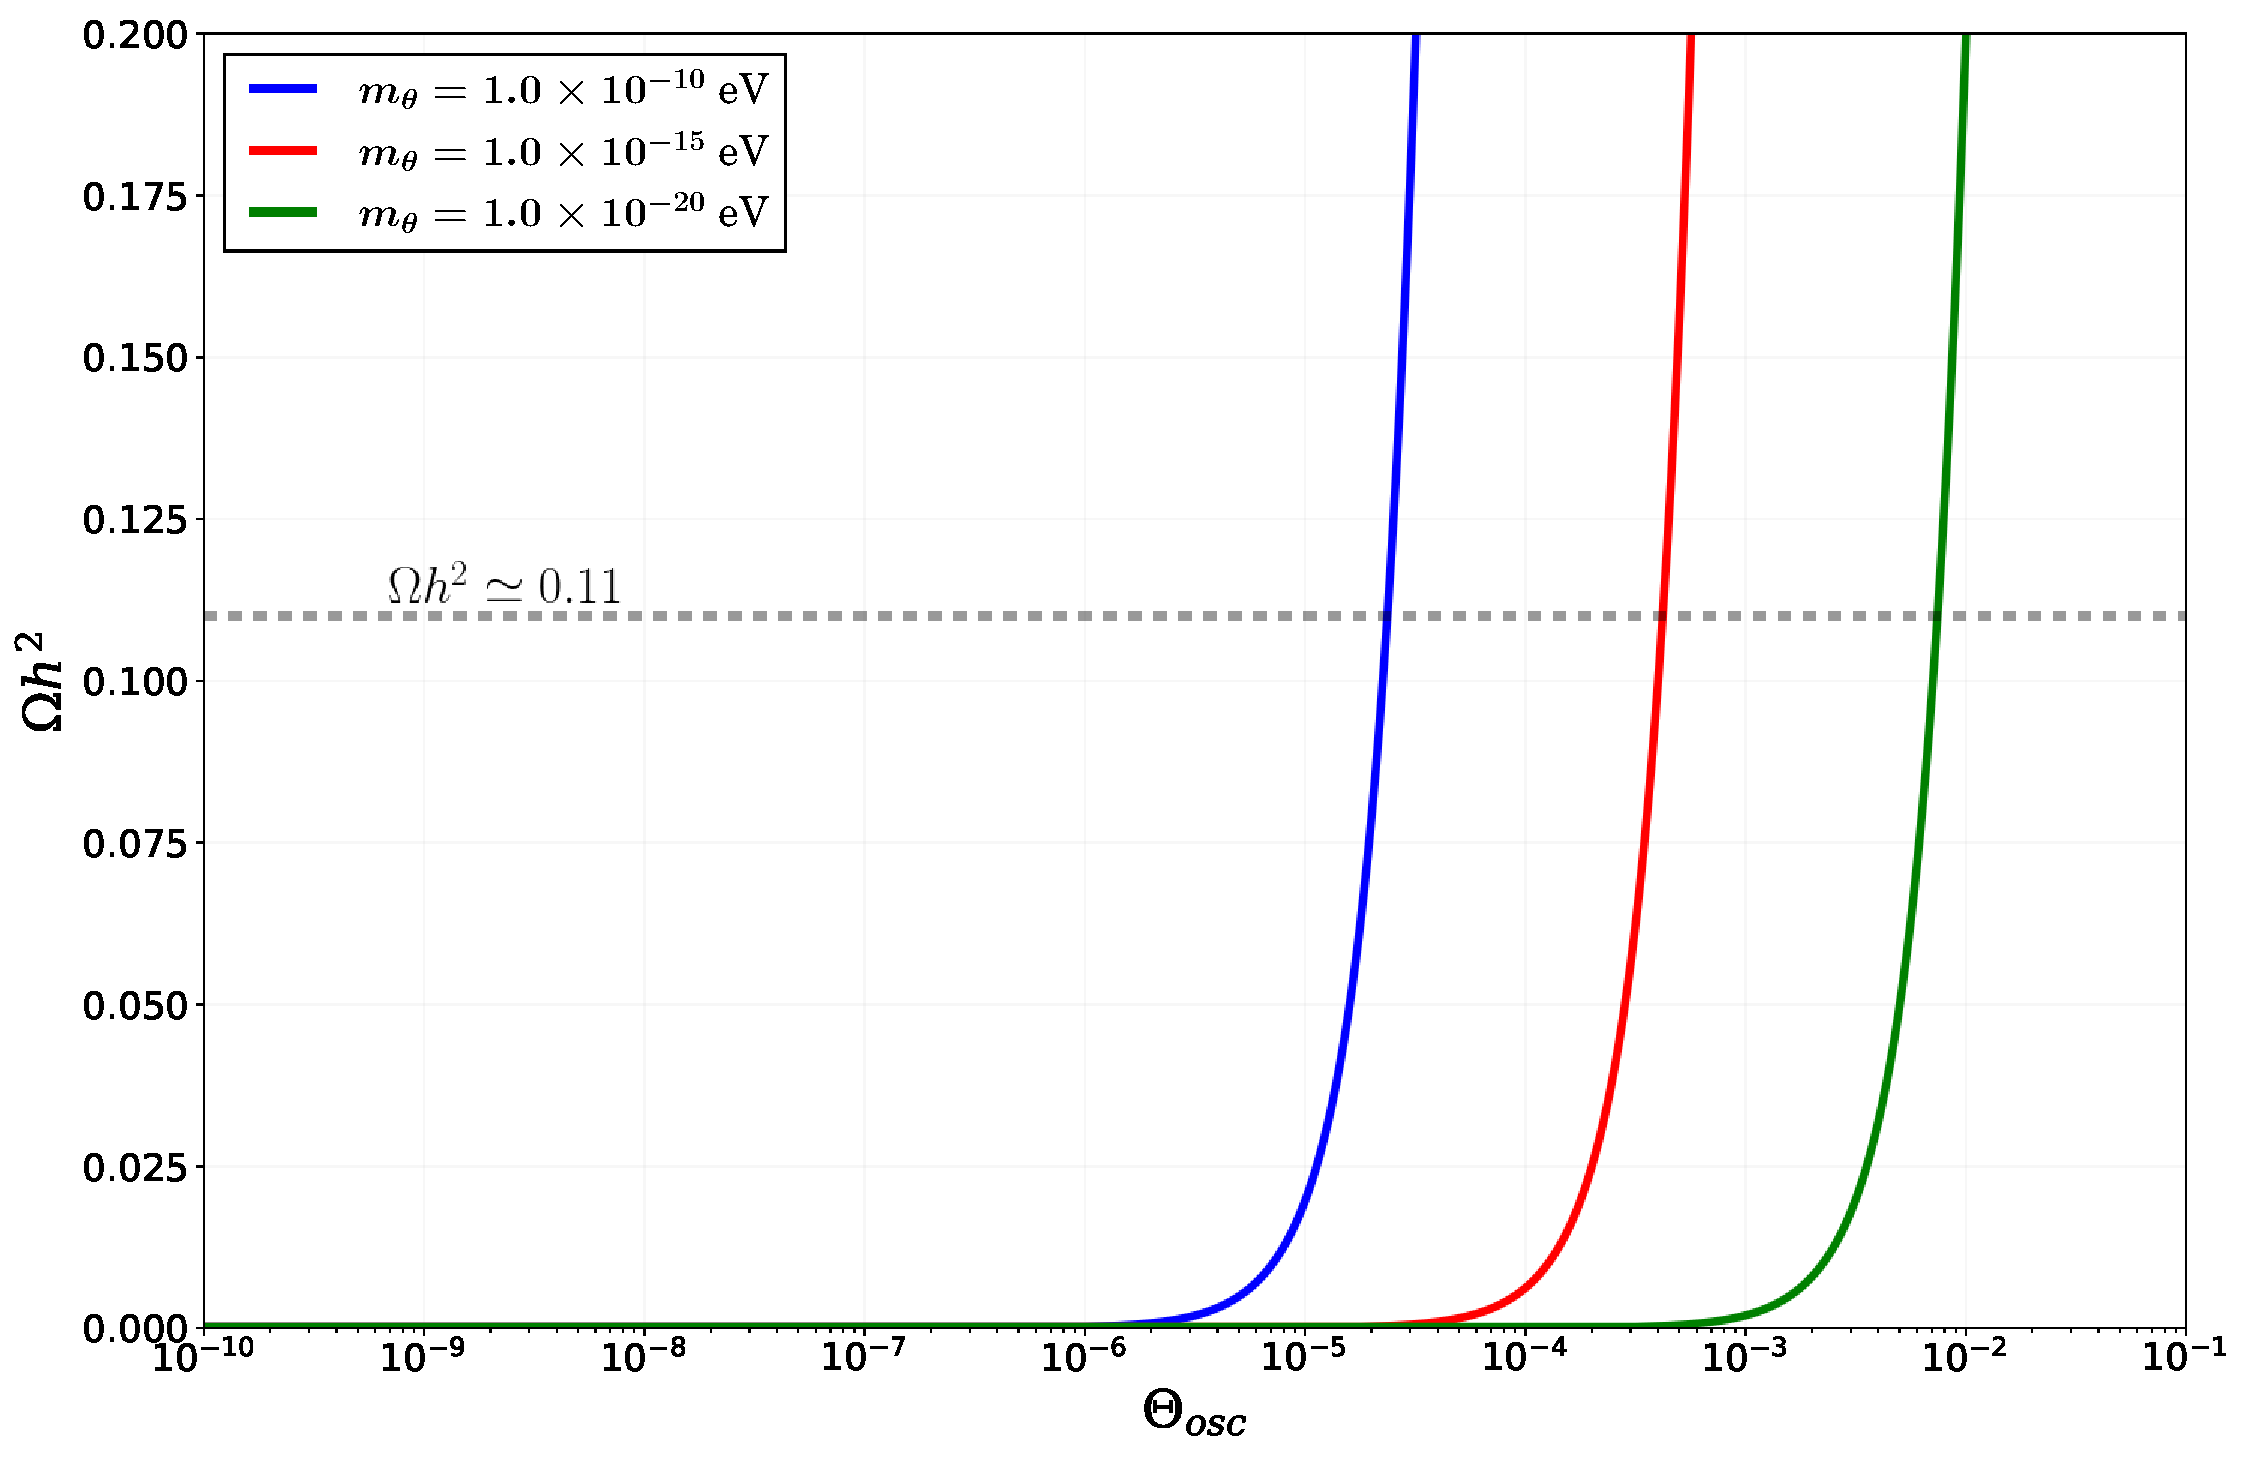
\includegraphics[width=0.9\linewidth]{graphs/relic_density.pdf}
	\caption{Relic density variating $\Theta_i$, with $v_\sigma=3\times 10^{18}$, for various values of $m_\theta$\,.}
	\label{fig:relicdesity}
\end{figure}

The \autoref{fig:relicdesity} allows us to determine the required initial misalignment angle, $\Theta_\textrm{osc}$, for certain mass and $v_\sigma$.